\section{Introducción}

El problema de filtraje consiste en estimar la trayectoria de un sistema dinámico, potencialmente estocástico, que se asume, en general, no completamente observable y con observaciones contaminadas por ruido. Este problema tiene aplicaciones en diversas áreas de la ingeniería y las ciencias, tales como análisis de señales, astronomía, mecánica de fluidos, procesamiento de imágenes médicas y, en el contexto de este trabajo, epidemiología y dinámicas de enfermedades infecciosas.

Los primeros avances matemáticos relacionados con el problema de filtraje fueron realizados de manera independiente por Wiener \cite{Wiener1949ExtrapolationSeries, M.1950TheApplications.} y Kolmogorov \cite{Kolmogorov1940StationarySpace}, quienes propusieron aproximaciones estadísticas de carácter general. Dichos desarrollos sentaron las bases de una línea de investigación que aborda el filtraje en múltiples aplicaciones matemáticas con la intención de proporcionar soluciones prácticas.

El primer enfoque algorítmico para el problema de filtraje fue introducido por Kalman \cite{Kalman1960AProblems}, quien desarrolló una metodología que, para el caso lineal, permite calcular de manera exacta la solución en tiempo discreto. Posteriormente, Kalman y Bucy extendieron este enfoque al caso continuo \cite{Kalman1961NewTheory}, dando lugar a los algoritmos conocidos como filtro de Kalman y filtro de Kalman-Bucy, respectivamente.

Tras resolver el caso lineal, surgió la necesidad de abordar el problema de filtraje en su forma no lineal. Sin embargo, se ha demostrado que una solución general requiere algoritmos de dimensión infinita, lo cual limita su implementación práctica en computadoras y restringe las soluciones disponibles a métodos subóptimos.

Con el objetivo de responder a las demandas de áreas que trabajan con modelos no lineales, se han desarrollado metodologías que ofrecen aproximaciones subóptimas al problema de filtraje. Entre estas destacan el filtro de Kalman extendido \cite{Smith1962ApplicationVehicle, McElhoe1966AnVenus} y el filtro de Kalman no lineal o Unscented Kalman Filter \cite{Julier2004UnscentedEstimation}. Aunque estas metodologías son extensiones del filtro de Kalman, en ciertos casos proporcionan soluciones insatisfactorias y carecen de propiedades asintóticas que garanticen la convergencia al óptimo.

Otra aproximación ampliamente utilizada es la de los filtros de partículas \cite{Hammersley1954PoorCarlo, Liu1998SequentialSystems}, los cuales emplean métodos de Monte Carlo para aproximar la solución, representada como una esperanza condicional, manteniendo la estructura secuencial del problema. Debido a su naturaleza asintótica, estos filtros, bajo ciertas condiciones sobre el sistema y el \textit{resampleo} de partículas, presentan cotas de error favorables para la solución del problema de filtraje \cite{Crisan2002APractitioners}.

En años recientes, se ha investigado la solución del problema de filtraje en espacios de Reproducing Kernel Hilbert Spaces (RKHS, por sus siglas en inglés). Estas estructuras, conocidas por sus aplicaciones en estadística, aprendizaje de máquinas y métodos numéricos \cite{Wendland2004ScatteredApproximation, Christmann2008SupportMachines}, ofrecen propiedades de interpolación y aproximación altamente valiosas. Entre los trabajos más relevantes en esta área destacan los de Fukumizu y Song \cite{Fukumizu2004DimensionalitySpaces, Song2009HilbertSystems}, quienes introdujeron la \textit{kernel Bayes rule}, una generalización de la regla de Bayes clásica adaptada a espacios de Hilbert.

De manera complementaria, los métodos basados en datos aplicados a sistemas dinámicos han encontrado en el operador de Koopman una herramienta poderosa. Introducido por Koopman y Von Neumann \cite{Koopman1931HamiltonianSpace, Koopman1932DynamicalSpectra}, este operador permite representar sistemas dinámicos no lineales de dimensión finita como sistemas lineales en dimensión infinita. Los avances de Mezić \cite{Mezic2013AnalysisOperator}, Schmid \cite{Schmid2008DynamicData}, Surana \cite{Surana2016KoopmanSystems}, Brunton \cite{Brunton2016KoopmanControl} y otros, han ampliado el uso del operador de Koopman en áreas como mecánica de fluidos, donde los datos disponibles permiten identificar dinámicas complejas.

El presente trabajo de tesis se encuentra en la intersección de estas tres áreas, contribuyendo con el desarrollo de un algoritmo de filtraje que integra el filtro de Kalman, los RKHS y el operador de Koopman, denominado \textit{kernel Koopman Kalman Filter} (kerKKF). Esta contribución se ilustra en la figura \ref{fig:venn_diagram}.

Asimismo, este trabajo profundiza en la conexión entre el filtro de Kalman y los RKHS, destacada como conexión 1 en la figura \ref{fig:conexiones}, enuncia y pruebas nuevos resultados de aproximación del operador de Koopman en RKHS, los que son usados posteriormente para establecer una cota de error para el algoritmo propuesto, representada como conexión 2. El objetivo principal es obtener una cota de error del orden $N^{-1/2}$, siendo $N$ la cantidad de puntos muestreados, lo cual sitúa este trabajo en un nivel comparable al de los filtros de partículas.

Por último, se incluyen resultados numéricos para modelos epidemiológicos, en particular variantes del modelo SIR clásico de Kermack y McKendrick \cite{Hethcote1989ThreeModels, Grassly2008MathematicalTransmission}, y se explora la aplicación del filtro en la estimación de parámetros, demostrando su versatilidad y precisión.

Esta tesis está organizada en cinco capítulos que se describen a continuación:

En el \textbf{Capítulo 2}, se presentan los preliminares necesarios para el desarrollo del trabajo. Este capítulo está enfocado en la exposición formal del problema de filtraje, incluyendo su formulación matemática detallada y una revisión de los algoritmos existentes en la literatura. Además, se abordan los aspectos fundamentales de los RKHS, esenciales para la comprensión del trabajo posterior y se presentan los modelos epidemiológicos que se utilizarán en los experimentos numéricos.

El \textbf{Capítulo 3} contiene los resultados obtenidos en el ámbito de \textit{kernel Extended Dynamic Mode Decomposition} (kEDMD), un método ampliamente estudiado en la literatura. En este capítulo, se utiliza dicha técnica para construir las herramientas necesarias para el diseño del filtro y la obtención de una nueva cota que es una alternativa a las cotas existentes en la literatura. El capítulo concluye con la presentación de resultados numéricos para casos lineales, así como para los modelos SIR, SIR con pérdida de inmunidad y SEIR.

En el \textbf{Capítulo 4}, se introduce el algoritmo \textit{kernel Koopman Kalman Filter} (kerKKF) en dimensión infinita, describiendo tanto su diseño como el análisis del error asociado a la aproximación del filtro mediante operadores de dimensión finita. Se expone la idea de que este filtro pertenece a una clase óptima de algoritmos que se basen en métodos de Monte Carlo y una generalización de la metodología para creación de filtros que utilicen una técnica de EDMD. También se detalla una metodología para la estimación de parámetros constantes en sistemas dinámicos. Este capítulo incluye resultados numéricos que demuestran la efectividad del filtro en sistemas lineales y en modelos epidemiológicos, además de resultados relacionados con la estimación de parámetros.

El \textbf{Capítulo 5} está dedicado a las conclusiones, discusiones y direcciones futuras de esta investigación. En este capítulo se analizan las posibles contribuciones de este trabajo al campo del filtraje, así como las formas en que podría ser mejorado y extendido en investigaciones futuras.

Por último, los códigos utilizados en esta investigación están disponibles en un repositorio público de \href{https://github.com/diegoolguinw/Koopman_nonlinear_filter}{GitHub}, donde también se proporcionan instrucciones sobre las dependencias necesarias. La implementación del algoritmo kerKKF ha sido empaquetada como una librería instalable mediante \texttt{pip}, cuyos detalles pueden encontrarse en el repositorio de \href{https://github.com/diegoolguinw/kkf}{GitHub}.

\begin{figure}[h]
    \centering
    \begin{subfigure}[b]{0.45\linewidth}
        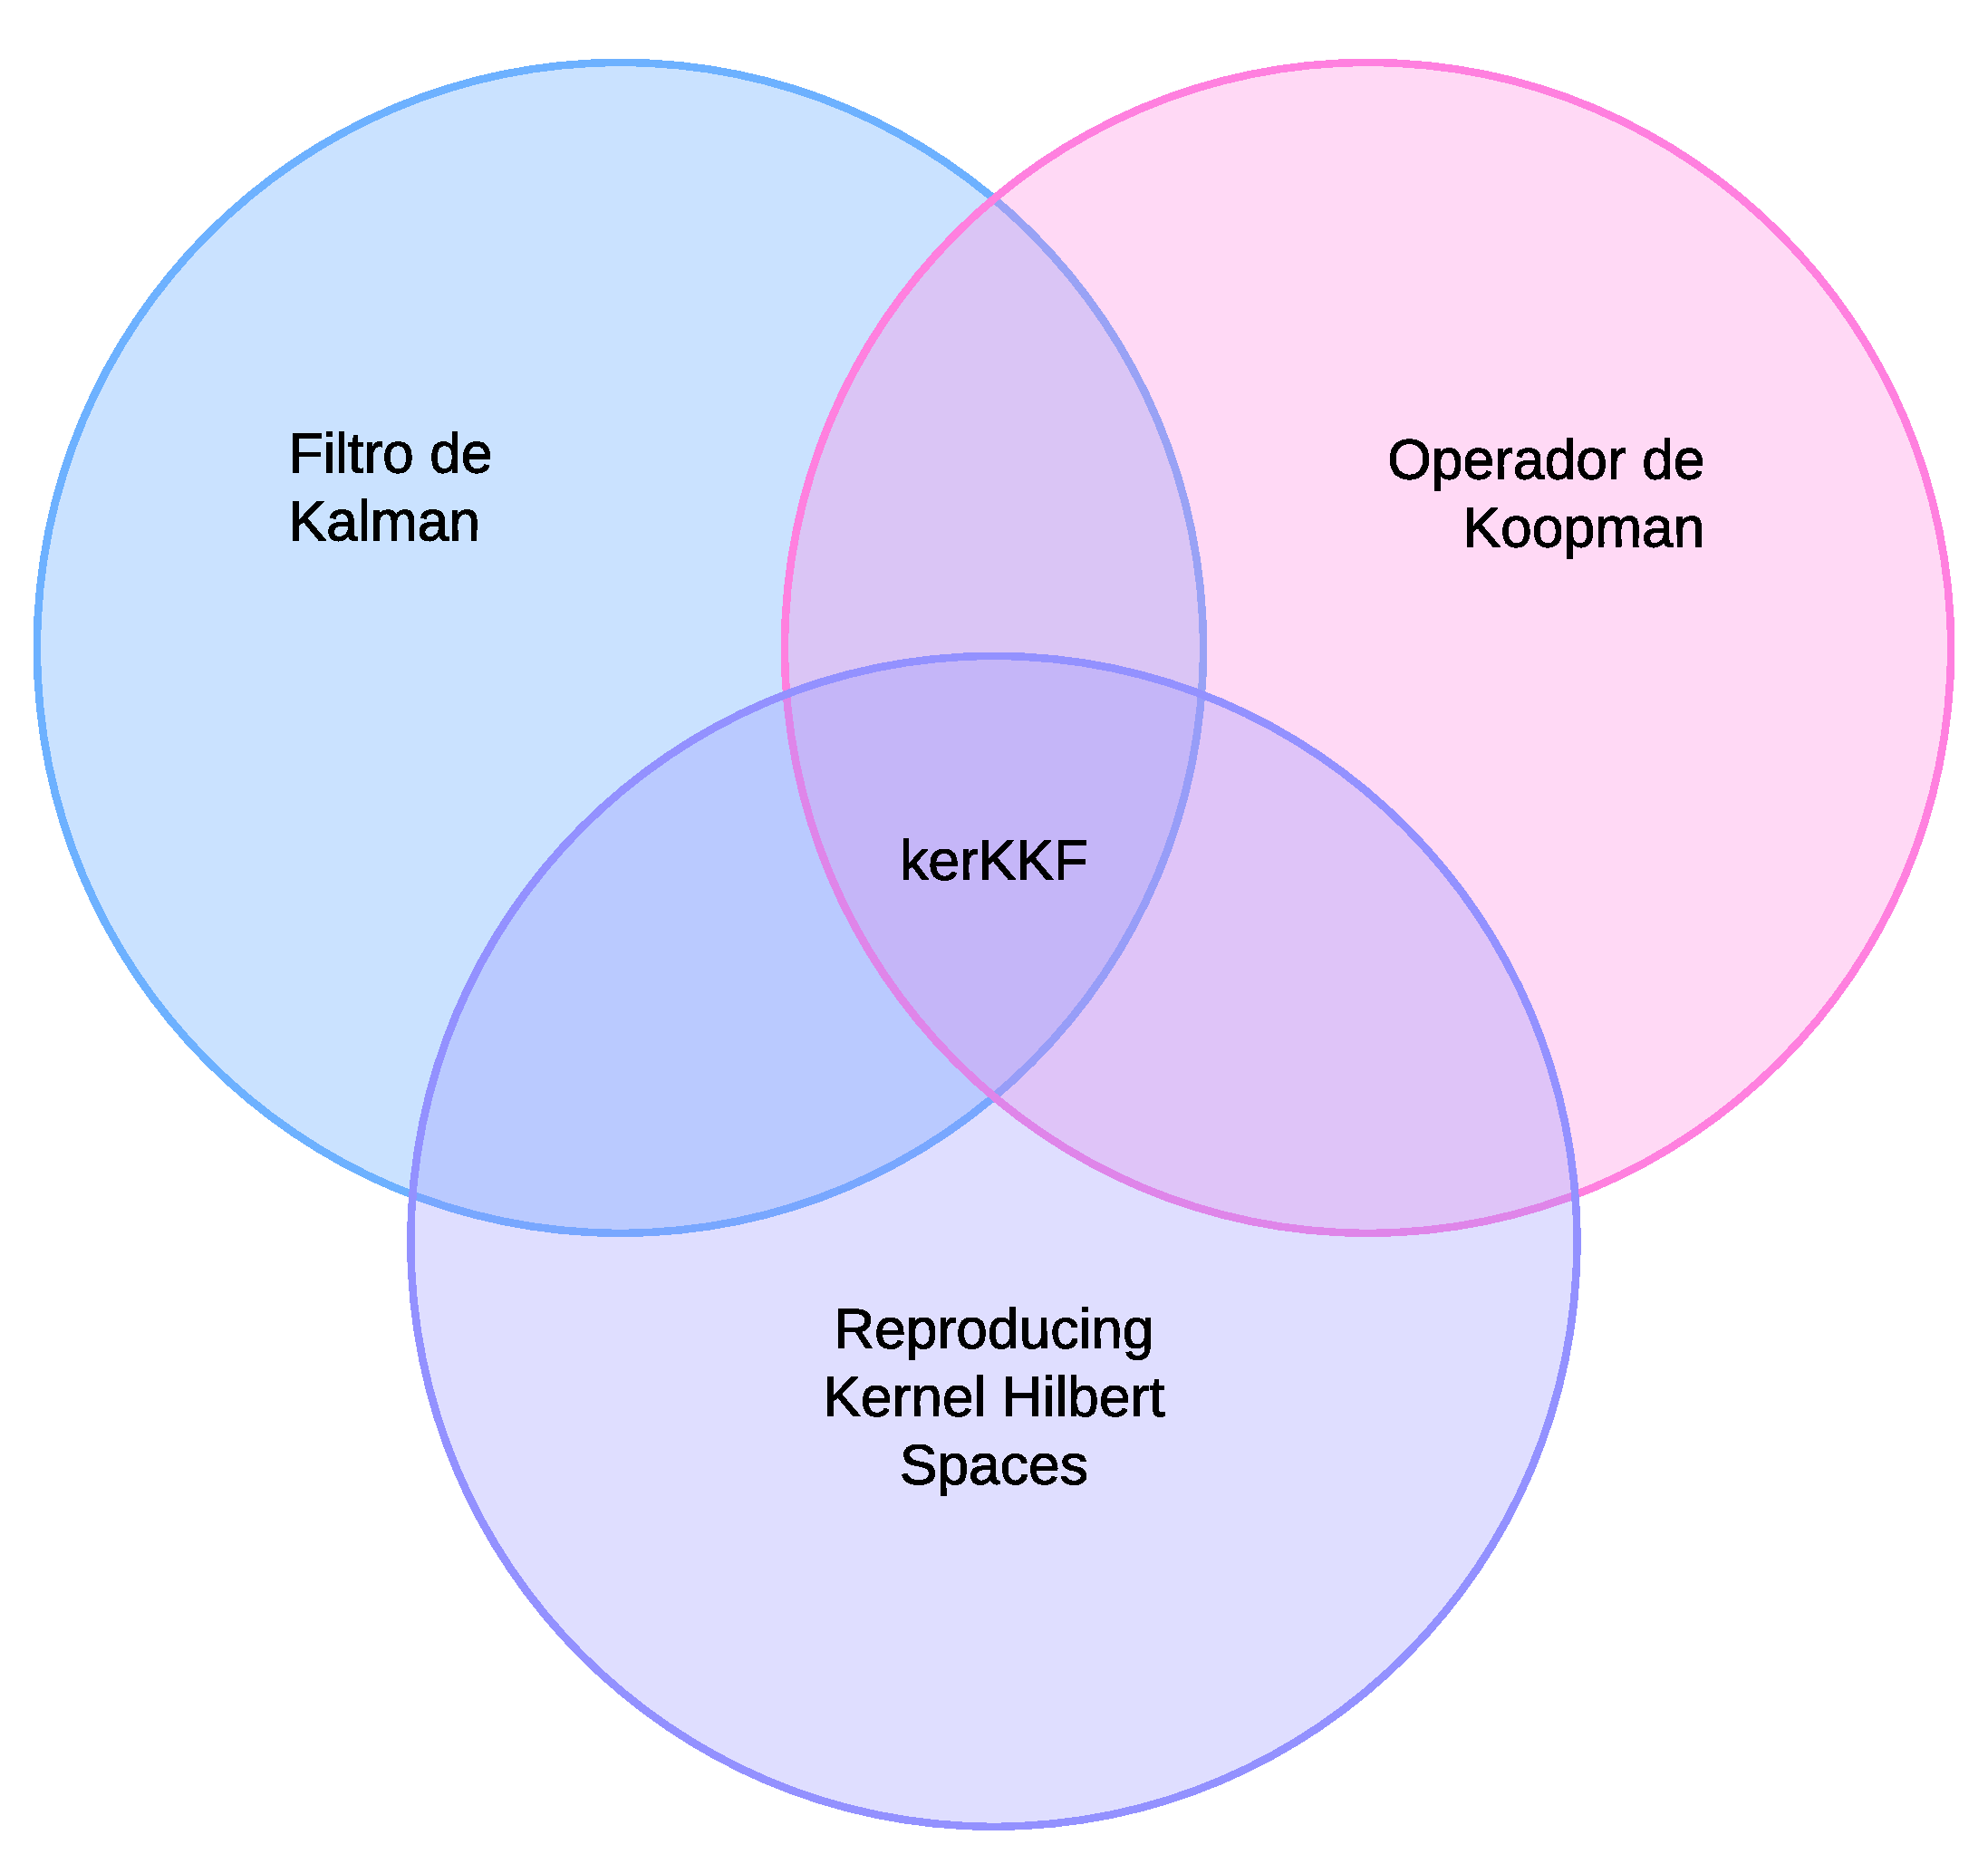
\includegraphics[width=0.9\linewidth]{img/content/chapter1/Venn_Diagram_Thesis.pdf}
        \caption{Diagrama de intersección de áreas como contribución de este trabajo.}
        \label{fig:venn_diagram}
    \end{subfigure}
    \begin{subfigure}[b]{0.45\linewidth}
        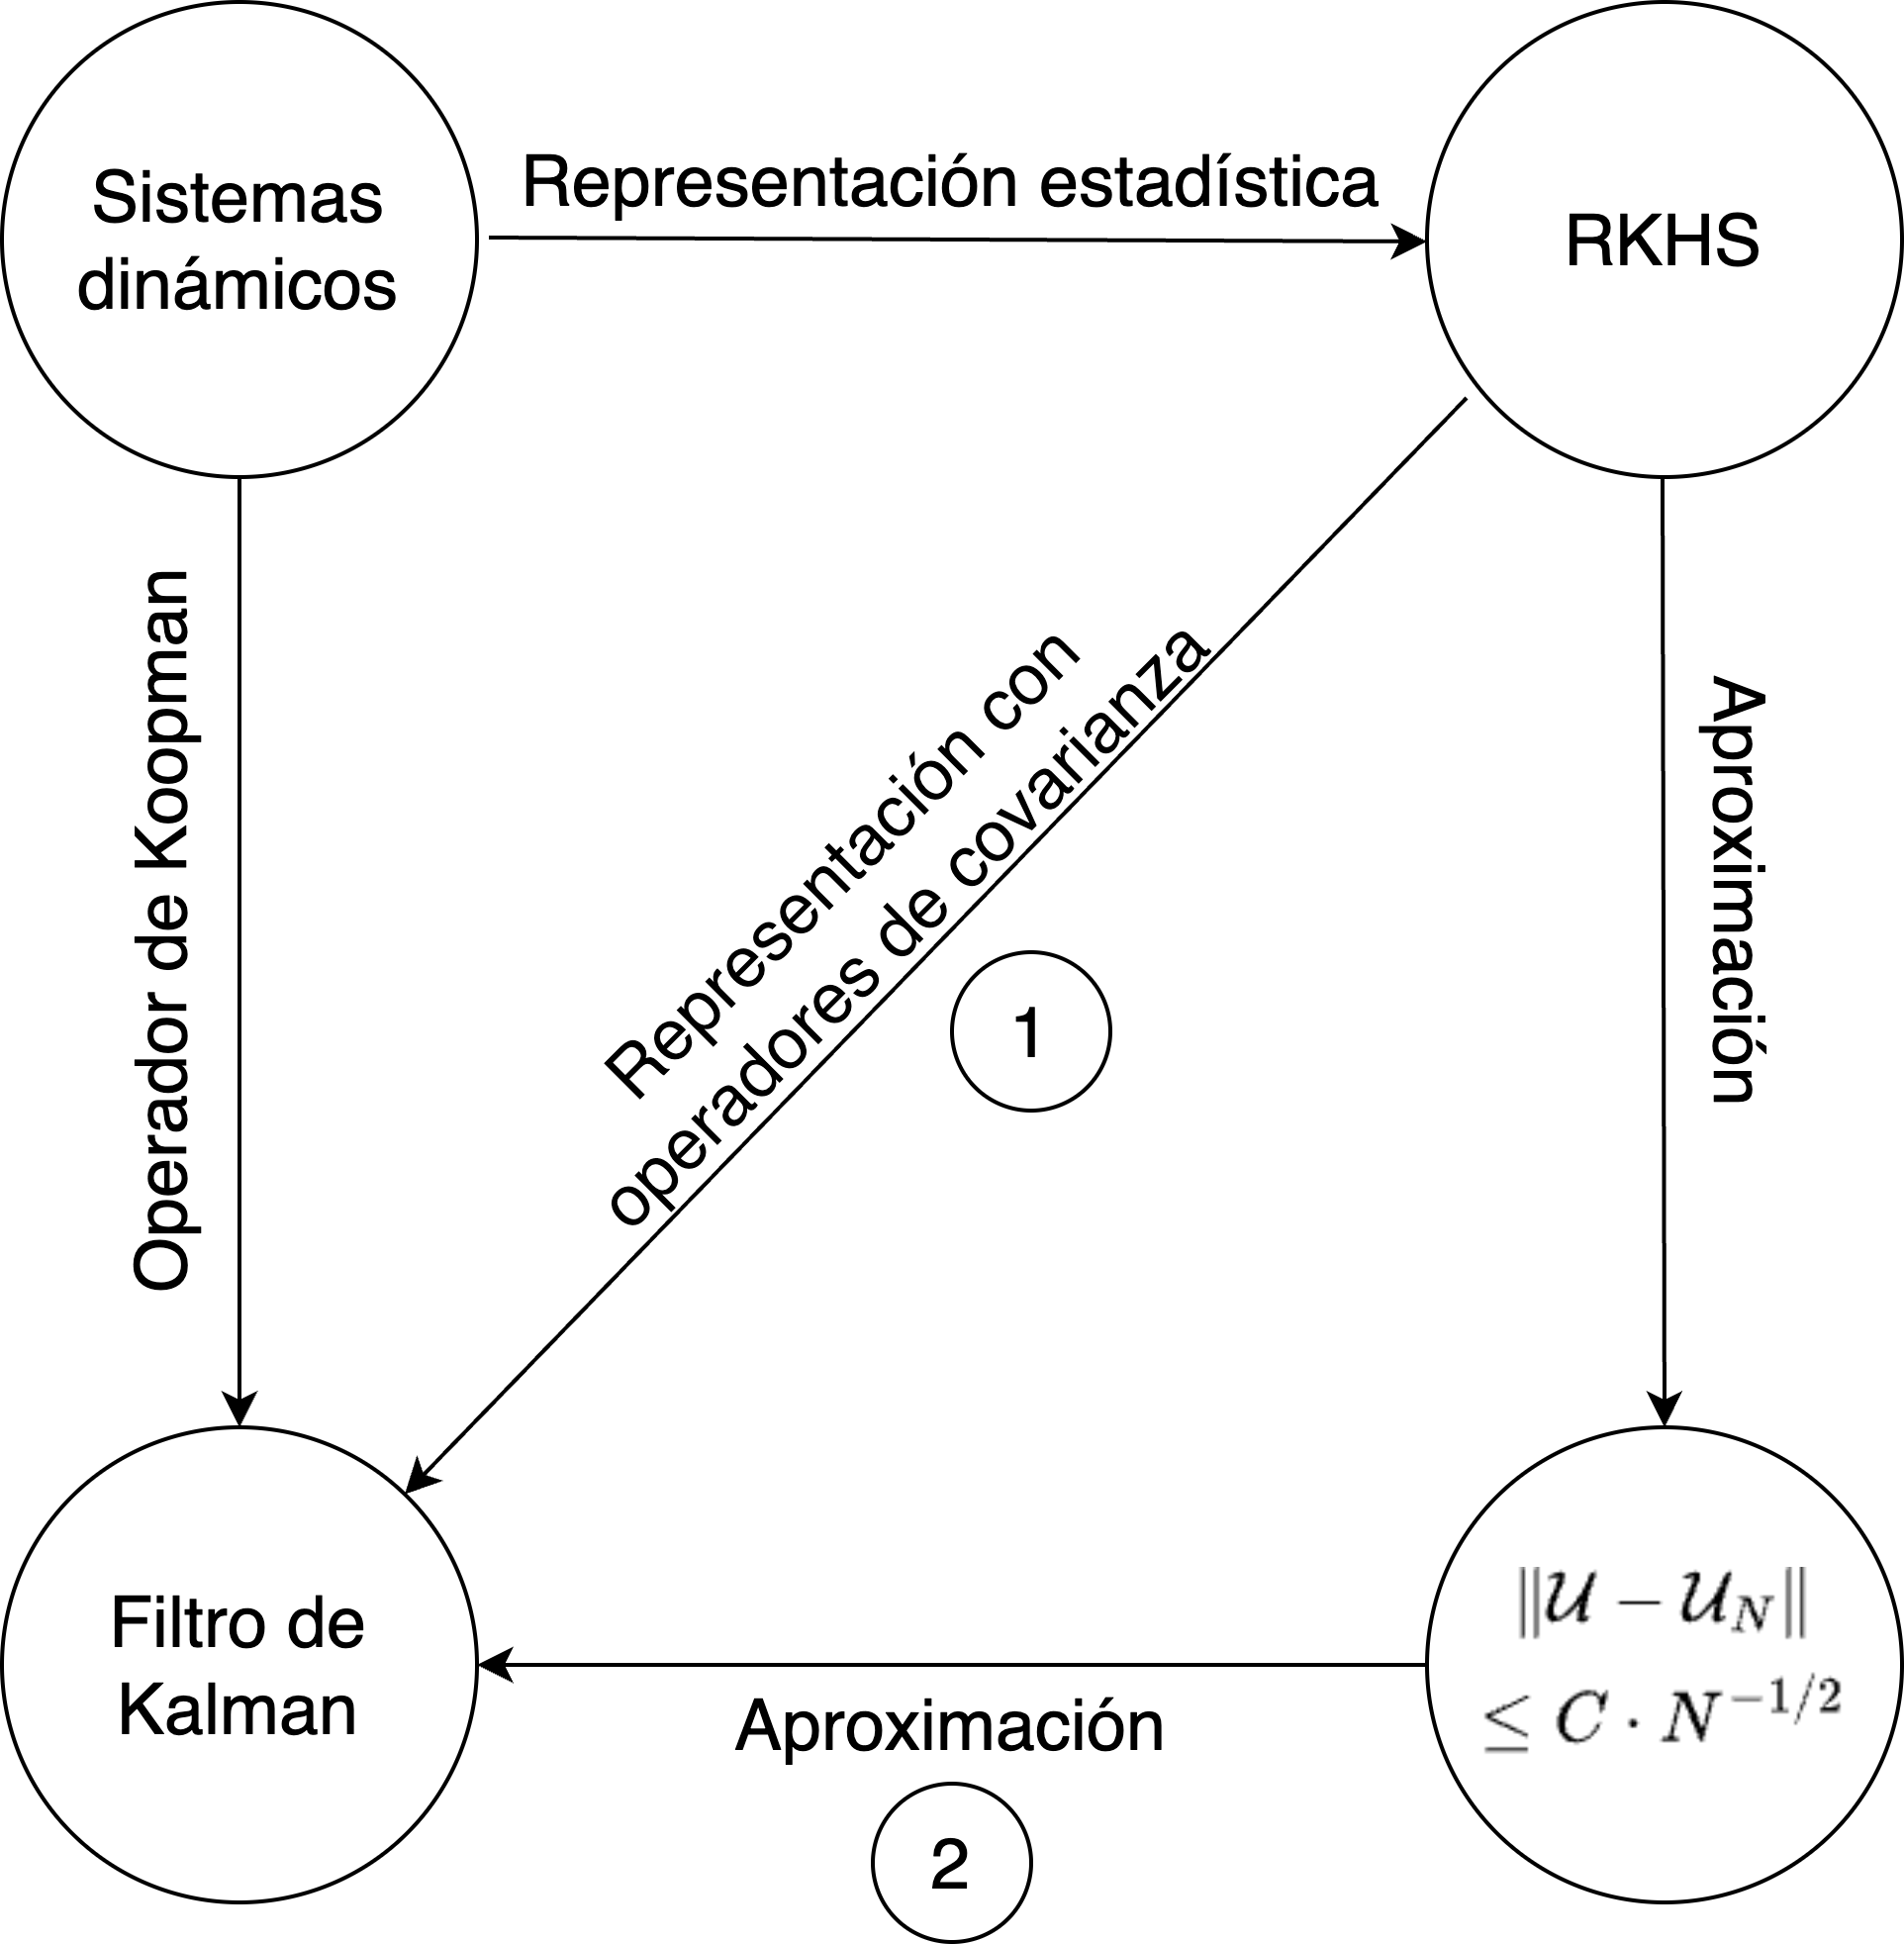
\includegraphics[width=0.9\linewidth]{img/content/chapter1/diag_contri.png}
        \caption{Diagrama de conexiones entre las áreas abordadas en este trabajo.}
        \label{fig:conexiones}
    \end{subfigure}
    \caption{Diagramas explicativos de las contribuciones de esta tesis.}
\end{figure}
